\newpage
\section{Handlungsanweisungen}
Im Folgenden werden Maßnahmen, die der Mitarbeitermotivation dienlich sind in drei Punkte unterteilt. Dabei werden sowohl Maßnahmen zur Motivationserhaltung als auch zur Motivationsförderung berücksichtigt. 
Im ersten Teil wird auf den Mitarbeiter als Individuum mit Gefühlen und Bedürfnissen eingegangen. Der zweite Teil konzentriert sich auf das Unternehmen als soziales Umfeld mit mehreren Mitarbeitern in einer hierarchischen Ordnung. Im dritten und letzten Teil liegt der Fokus auf dem Unternehmen als Arbeitsumfeld.

Alle drei Unterpunkte konzentrieren sich dabei auf geistig anspruchsvolle Tätigkeiten. Das bedeutet, dass insbesondere die Maßnahmen der Belohnung und deren Höhe, bei primitiven Tätigkeiten eine andere Wirkung erzielen können, als im Folgenden beschrieben. 

Allen drei Unterpunkten folgt nach der Aufführung der Maßnahmen und ihrer Wirkung eine Wirtschaftlichkeitsbetrachtung. Diese soll dabei unterstützen, ein vertretbares Maß zwischen Wirkung und Wirtschaftlichkeit zu finden. 

\subsection{Mitarbeiter als Individuum}
In den folgenden Abschnitten werden die einzelnen Unterpunkte beleuchtet, die den Mitarbeiter als Individuum betreffen.

\subsubsection{Mitarbeiter als Mensch}
Jeder Mitarbeiter ist in erster Linie ein Mensch, der mit Emotionen und Gefühlen, sowie Bedürfnissen ausgestattet ist. Nach \citet[S. 18]{Seelbach.2011}  stimuliert den Menschen nichts mehr als der Wunsch wahrgenommen zu werden, das umfasst die Aussicht auf soziale und zwischenmenschliche Anerkennung, Wertschätzung und Zuwendung. 
Der Wunsch nach Wahrnehmung kann z.B. damit bedient werden, dass der Mitarbeiter in regelmäßigen Abständen persönlich angesprochen wird. Bereits mit einfachen Worten wie einem Lob oder einem \glqq Danke\grqq d.h. die Wertschätzung geleisteter Arbeit zu hohem Maß motivieren kann. Darüberhinaus läuft die Kommunikation bidirektional, d.h. man sollte dem Mitarbeiter auch zuhören, die Chance geben sich mitteilen zu können. 
Die Bedürfnisse der Menschen sind unterschiedlich, deswegen gilt es eher eine maßgeschneiderte Zuwendung zu versuchen statt einer Gleichbehandlung. 

\subsubsection{Entlohnung}
Die Wertschätzung eines Mitarbeiters drückt sich auch in dessen Gehalt aus. Es ist ein Ausdruck der Entlohnung seiner Fähigkeiten und Zeit. Das bedeutet im Umkehrschluss, dass ein niedriges Gehalt als eine Geringschätzung der Arbeit eines Mitarbeiters oder gar dessen selbst gewertet wird. Generell ist das monatliche Gehalt nicht als Motivator zu sehen, da hierbei sehr schnell der in 3.2 beschriebene Lerneffekt einsetzt und es somit als normal empfunden wird.

Bei der Mitarbeitergewinnung ist das Gehalt ein primärer Anreiz der einem Bewerber angeboten werden kann. Aussicht auf Erfolg besteht dabei nur, wenn der Betrag die Bedürfnisbefriedigung erlaubt und im Vergleich mit anderen Stellen bzw. Unternehmen als gerecht empfunden wird. Geht mit einem Unternehmenswechsel ein merkbarer Gehaltsanstieg einher, so unterliegt auch dieser einem Lerneffekt (siehe 3.2), was dazu führt, dass das höhere Gehalt schon nach kurzer Zeit als normal empfunden wird.

\subsubsection{Tätigkeitsbild}
Der Mensch ist keine Maschine. Diese Aussage ist seit Anfang des 20. Jahrhunderts und spätestens durch Charlie Chaplins Film \glqq Moderne Zeiten\grqq \cite{Chaplin.1936} einer breiten Masse bekannt. 
Mit der Aufnahme einer beruflichen Tätigkeit nach der Ausbildung sind viele Erwartungen und Hoffnungen verknüpft, stellt sie doch einen der wichtigsten Schritte im Leben eines Menschen dar.  
Im Rahmen einer aktuellen Umfrage \citep{Allensbach.2014} unter Studenten wurde unter anderem nach den Erwartungen und Hoffnungen an die eigene zukünftige berufliche Tätigkeit gefragt. Die Antworten der Studenten waren äußerst vielfältig und nicht \glqq primär an materiellen Gratifikaten ausgerichtet\grqq. Mit einem signifikaten Abstand von über 20 \% stehen auf den ersten Plätzen weiche Faktoren. Auf Platz Platz 1 liegt für 73\% der Studenten, der Wunsch nach einem “guten Betriebsklima”. Danach kommt mit 67\% ein “sicherer Arbeitsplatz” und mit 66\%, dass die Tätigkeit kongruent mit den eigenen Fähigkeiten und Neigungen ist. Auf dem vierten Platz kommt für 65\%, dass die Vereinbarkeit zwischen Privatleben und Beruf funktioniert. Erst auf dem 7.Platz kommt ein “hohes Einkommen”.

\begin{figure}[!h]
\centering
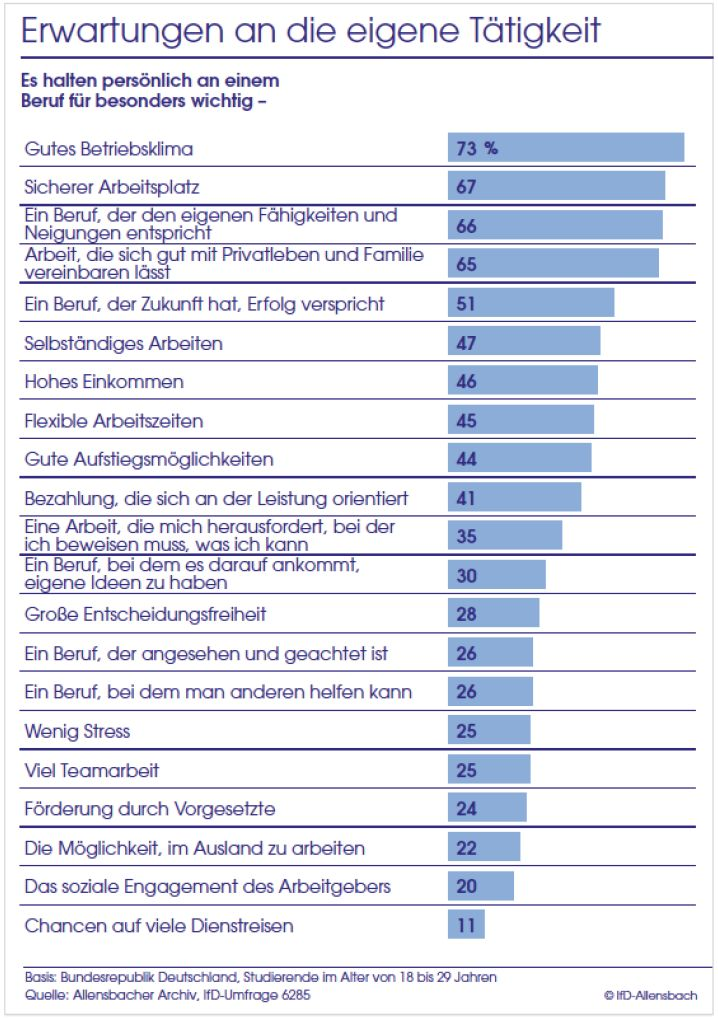
\includegraphics[width=0.8\linewidth]{grafiken/abb4.jpg}
\caption{Umfrageergebnisse der Studie, \newline Quelle: \cite[S. 53]{Allensbach.2014}}
\label{fig:Gehirn4}
\end{figure}

Die Studie zeigt, wie wichtig eine angemessene Tätigkeit ist. Eine abwechslungsreiche, herausfordernde, aber nicht überfordernde, Tätigkeit, die den eigenen Qualifikationen und Neigungen entspricht, bringt das höchste Motivationspotential mit. 
Die Freiheit bei der Erledigung der Aufgaben kann z.B. durch Zielvorgaben anstatt detaillierte Arbeitsanweisungen erreicht werden. 
Müssen unbeliebte Tätigkeiten erledigt werden, kann mit Inaussichtstellung einer besonders spannenden Tätigkeit motiviert werden. 

\subsubsection{Belohnung}
Zur Leistungserhaltung, aber vor allem zur Leistungssteigerung dienen Anreize in Form von Belohnungen. Generell sollte eine Belohnung dabei in Relation zur erbrachten Leistung stehen. Dabei entfaltet die Ankündigung einer Belohnung dieselbe Wirkung wie die Vergabe einer solchen. Das lässt sich nutzen, um zum Beispiel für die Erledigung einer weniger spannenden Aufgabe, dafür eine umso Interessantere danach in Aussicht zu stellen. 

Bei einer leistungsbezogenen Belohnung spielen zwei Faktoren eine große Rolle für die Wirksamkeit dieser auf die Motivation eines Mitarbeiters. Zum einen muss der Mitarbeiter Einfluss auf die Erreichung der gesetzten Ziele haben. So wird in einem großen Unternehmen der einzelne Sachbearbeiter nur einen sehr geringen Einfluss auf den Jahresgewinn haben. Ein Vertriebsmitarbeiter hingegen, der eine Provision auf seine Verkäufe erhält, hat maßgeblichen Einfluss darauf.
Zweiter wichtiger Faktor ist der Zeitpunkt des Erhalts der Belohnung. Liegt dieser in weiter Ferne, wird der Erhalt als risikoreicher empfunden und somit die Wirkung deutlich geringer ausfallen.

Eine zu hohe Belohnung bewirkt u.U. das Gegenteil der gewünschten Leistungssteigerung (siehe 3.2). Bei jeglicher Form der Belohnung sollte darauf geachtet werden, dass diese bei regelmäßiger Anwendung einem Lerneffekt unterliegen, welcher ihre Wirkung maßgeblich beeinflussen kann. So wird eine jährliche Sonderleistung wie z.B. das in Deutschland weit verbreitete Urlaubsgeld schon nach wenigen Jahren als normal empfunden. Damit wird bereits ein einmaliger Ausfall als Verlust empfunden. Eine Gegenmaßnahme sind unerwartete Belohnungen. Diese unterliegen ebenso dem Lerneffekt, wirken aber grundsätzlich viel stärker (siehe 3.2). 

Direkte Belohnungen wirken in den meisten Fällen deutlich besser als Abstrakte. Geld als bekannteste abstrakte Belohnung hingegen benötigt ein zugrunde liegendes Bedürfnis, welches sich damit befriedigen lässt.

Der größte Demotivator hingegen sind falsche Versprechungen, wenn also eine angekündigte Belohnung ausfällt. Dies führt zu negativen Emotionen wie Wut und Frustration. Vor allem bei mehrfachen Fällen geht damit die gesamte Wirkung einer Belohnungsankündigung verloren (siehe 3.2). Daher sollte in Fällen, bei denen der Erhalt der Belohnung nicht sicher ist, auf eine Ankündigung dieser verzichtet werden, und statt dessen auf den Effekt einer unerwarteten Belohnung im Nachhinein genutzt werden. 

\subsubsection{Wirtschaftlichkeitsbetrachtung}
Bereits mit Wertschätzung und Anerkennung der Leistung eines Mitarbeiters ist oft schon viel erreicht. Ein einfaches Lob und ein Dankeschön kosten kein Geld, haben aber eine nicht zu vernachlässigende Wirkung (siehe 4.1.1). Ebenso kann mit direkten, auf die Bedürfnisse des Mitarbeiters zugeschnittenen Belohnungen in vielen fällen eine größere Wirkung erreicht werden, als mit einer hohen Bohnuszahlung (siehe 4.1.4). Als Beispiel sei hier eine Bahncard genannt, die Mitarbeiter auch privat nutzen kann. 
Natürlich kann nicht jeder Wunsch eines Mitarbeiters berücksichtigt werden. Der notwendige Verwaltungsaufwand wäre unüberschaubar hoch. Jedoch kann wie oben beschrieben mit einfachen, und im Idealfall unbürokratischen, Mitteln, mit weniger finanziellem Aufwand oft mehr erreicht werden. 

Bei den Kosten gilt es neben den kurzfristigen Mehraufwendungen auch die langfristigen Einsparungen zu beachten, dazu zählen z.B. Ausfall von Mitarbeitern durch Krankheit. Nach \citet{Schlolaut.2013} können Unternehmen es sich nicht dauerhaft leisten, ihre Mitarbeiter zu erschöpfen. Der dadurch entstehende wirtschaftliche Schaden für die Unternehmen und für die Gesellschaft ist unübersehbar. Ein weiterer Faktor ist die Vermeidung der “Sinnlosigkeit des eigenen Tuns”. Dazu zählen plötzlich abgebrochene Projekte oder unangemessene Aufgaben, die nichtersichtliche Gründe haben.

\subsection{Unternehmen als soziales Umfeld}
Ein Unternehmen ist ein soziales Umfeld bestehend aus mehreren Mitarbeiter, in welchem eine Vielzahl von sozialen Einflüssen auf die Motivation der Mitarbeiter wirkt. 

\subsubsection{Gerechtigkeitsprinzip}
Die Belohnung von Mitarbeitern in einem Unternehmen ist eine Aufgabe, bei der es mehrere Punkte zu beachten gilt. Die gezielte Belohnung eines Einzelnen kann von Anderen als eine Bestrafung empfunden werden. Dies betrifft jedoch nicht nur Belohnungen im monetären oder materiellen Sinn, sondern erstreckt sich auch auf soziale Anerkennung und Interaktion (siehe 3.2.6). \glqq Für die Führungspraxis bedeutet das: Wer Menschen nachhaltig führen und motivieren will, muss ihnen die Möglichkeit geben, mit anderen zu kooperieren und Beziehungen zu gestalten.\grqq \cite[S. 18]{Seelbach.2011} 

In Deutschland wird überlicherweise nicht über das Gehalt gesprochen. Bei nicht-tarifgebundenen Unternehmen sollte daher ein Gehaltsrahmen definiert werden, der transparente Gehaltsgruppen festlegt. Diese sollten Erfahrung und Tätigkeit eines Mitarbeiters berücksichtigen und somit auf der einen Seite Spielraum für seine individuelle Leistung geben und auf der anderen Seite für ein ausreichendes Maß an Gerechtigkeit zwischen allen Mitarbeitern sorgen. 

\subsubsection{Wirtschaftlichkeitsbetrachtung}
Um die in 4.1.4 genannten Möglichkeiten der individuellen Belohnung in einem transparenten Gehaltsrahmen berücksichtigen zu können, wird im Folgenden anhand des Cafeteria-Modells gezeigt.

Das Cafeteria-Modell wird anhand der drei folgenden Komponenten umgesetzt: einem Budget, einer periodischen Wahlmöglichkeit und einem Wahlangebot.
Der Vorteil ist, dass das Unternehmen ein festes Budget einplanen kann, das pro Periode für dieses Anreizsystem zur Verfügung steht. Der Mitarbeiter kann seine persönlichen Bedürfnisse gezielt befriedigen, ohne dass eine zeitaufwändige Analyse durch eine dritte Person erfolgt. Dadurch entsteht ein hoher Wirkungsgrad. Das dem Mitarbeiter zur Verfügung stehende Budget kann durch besondere Leistungen erweitert werden.
Gleichzeitig wird die Gerechtigkeit durch einen allgemein verbindlichen Rahmen gewährleistet. Das Zusammengehörigkeitsgefühl kann dadurch auch gestärkt werden, indem z.B. gemeinsam Aktivitäten ausgeübt werden können. Ein Nachteil für das Unternehmen ist beim Cafeteria-Modell der zusätzliche Verwaltungsaufwand. Auf der einen Seite müssen die Mitarbeiter nicht mehr analysiert werden, auf der anderen Seite ist jedoch das Management der einzelnen \glqq Wahlangebote\grqq mit einem gewissen Aufwand verbunden (z.B. Vertragslaufzeiten der Bahncard usw.).
Je nach Land, z.B. in Deutschland, ist auch die steuerrechtliche Grundlage kompliziert. 
Davon abgesehen können über das Cafeteria-Modell nur monetär abbildbare Werte angeboten werden. \cite[S. 55ff]{Nowka.2013}

\subsection{Unternehmen als Arbeitsumfeld}
Das Unternehmen bietet seinen Mitarbeitern einen Arbeitsplatz zur Erbringung ihrer Arbeitsleistung. 

\subsubsection{Anreize im Arbeitsumfeld}
Die Gestaltung des Arbeitsumfelds bietet vielfältige Möglichkeiten zur Anreizgestaltung. Angefangen bei der individuellen Arbeitsplatzausstattung über Gemeinschaftsräume wie Pausenraum bis zu Wohlfühlfaktoren wie kostenlosen Heiß- und Kaltgetränken sind hier einem Unternehmen keine Grenzen gesetzt. Ziel dieser Maßnahmen ist es, den Aufenthalt der Mitarbeiter am Arbeitsplatz so angenehm wie möglich zu gestalten. Dabei sind auch Kooperationen mit anderen Unternehmen plausibel, wie das Beispiel unternehmensübergreifender Kindertagesstätten zeigt. 

All diese Anreize können bei der Mitarbeitergewinnung als zusätzliche Vorteile angeführt werden. Sie fördern die Motivation  Längerfristige Maßnahmen wie Betriebskindertagesstätten fördern darüber hinaus die Mitarbeiterbindung. 

In erster Linie bei der Arbeitsplatzausstattung gilt jedoch auch ein Mindestmaß, welches Mitarbeiter zur Erledigung ihrer Arbeit als Voraussetzung sehen. Wird dieses nicht erfüllt, so entsteht sehr schnell Frustration. Ebenso unterliegen alle oben genannten Formen von Anreizen einem Lern- bzw. Gewöhnungseffekt. Sind die Mitarbeiter es gewohnt, kostenlose Getränke am Arbeitsort zu erhalten, wird ein Wegfallen dieser Leistung als Verlust wahrgenommen und führt somit ebenfalls zu Demotivation und fördert Frustration. Daher sollte bei Einführung dieser Maßnahmen darauf geachtet werden, dass diese in erster Linie nicht der kurzfristigen Förderung der Mitarbeitermotivation dienen, sondern viel mehr dem langfristigen Erhalt der Motivation.

\subsubsection{Wirtschaftlichkeitsbetrachtung}
Generell ist bei der Arbeitsumgebung darauf zu achten, dass der als üblich erachtete Mindeststandard erfüllt werden kann, damit diese nicht demotivierend wirkt. Eine Erhöhung des Standards bringt zwar die bereits beschäftigten Mitarbeiter nur einen kurzzeitigen Motivationsschub, kann jedoch als positiver Anreiz für die Mitarbeitergewinnung genutzt werden. Wichtig ist hier sich an den Standards der eigenen Branche zu orientieren. Werden Maßnahmen wie kostenlose Getränke für alle Mitarbeiter eingeführt, sollte bei der Einführung auf jeden Fall darauf geachtet werden, dass eine Abschaffung dieser mit einer hohen Demotivation der Mitarbeiter einhergeht.